\documentclass[journal]{IEEEtran}

\usepackage[T1]{fontenc}% optional T1 font encoding

\usepackage[pdftex]{graphicx}

\ifCLASSOPTIONcompsoc
\usepackage[caption=false,font=normalsize,labelfon
t=sf,textfont=sf]{subfig}
\else
\usepackage[caption=false,font=footnotesize]{subfi
g}
\fi

\begin{document}

\begin{figure*}
\centering
\subfloat[Target reconstruction.]{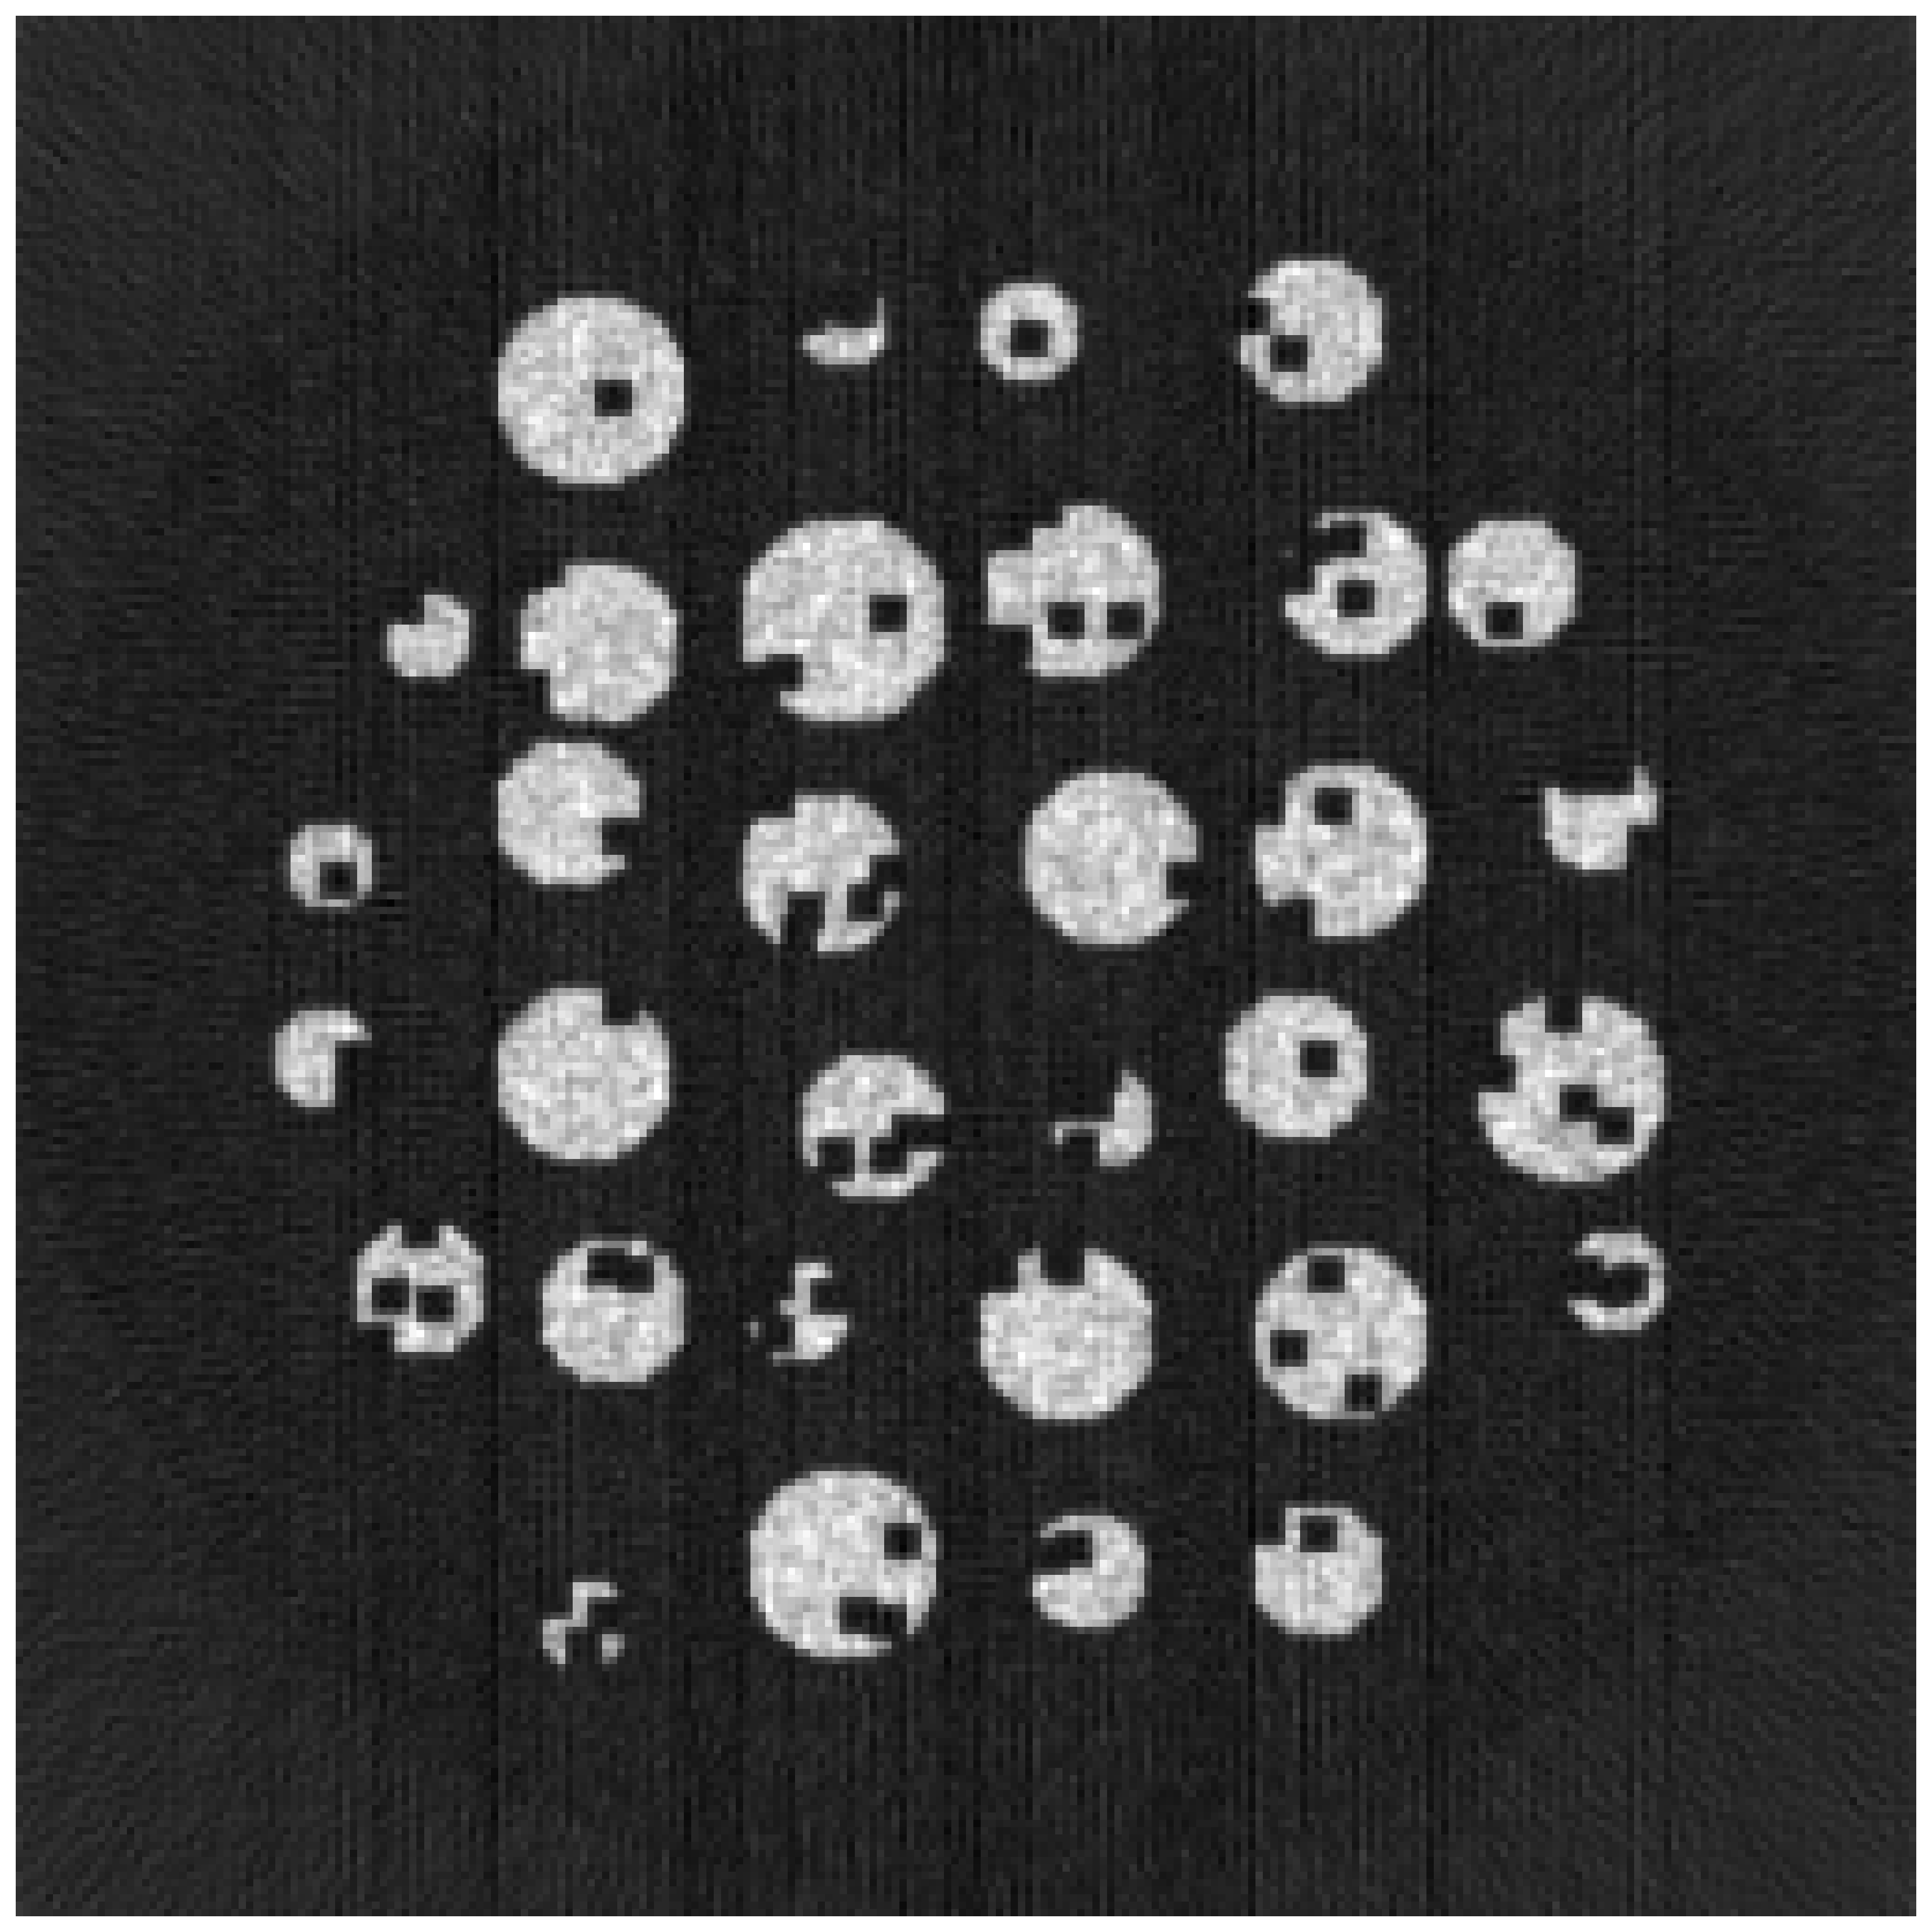
\includegraphics[width=0.15\textwidth]{ holes_tar.png}
\label{fig:holes_tar}}
\hfill
\subfloat[Reconstruction using our method.]{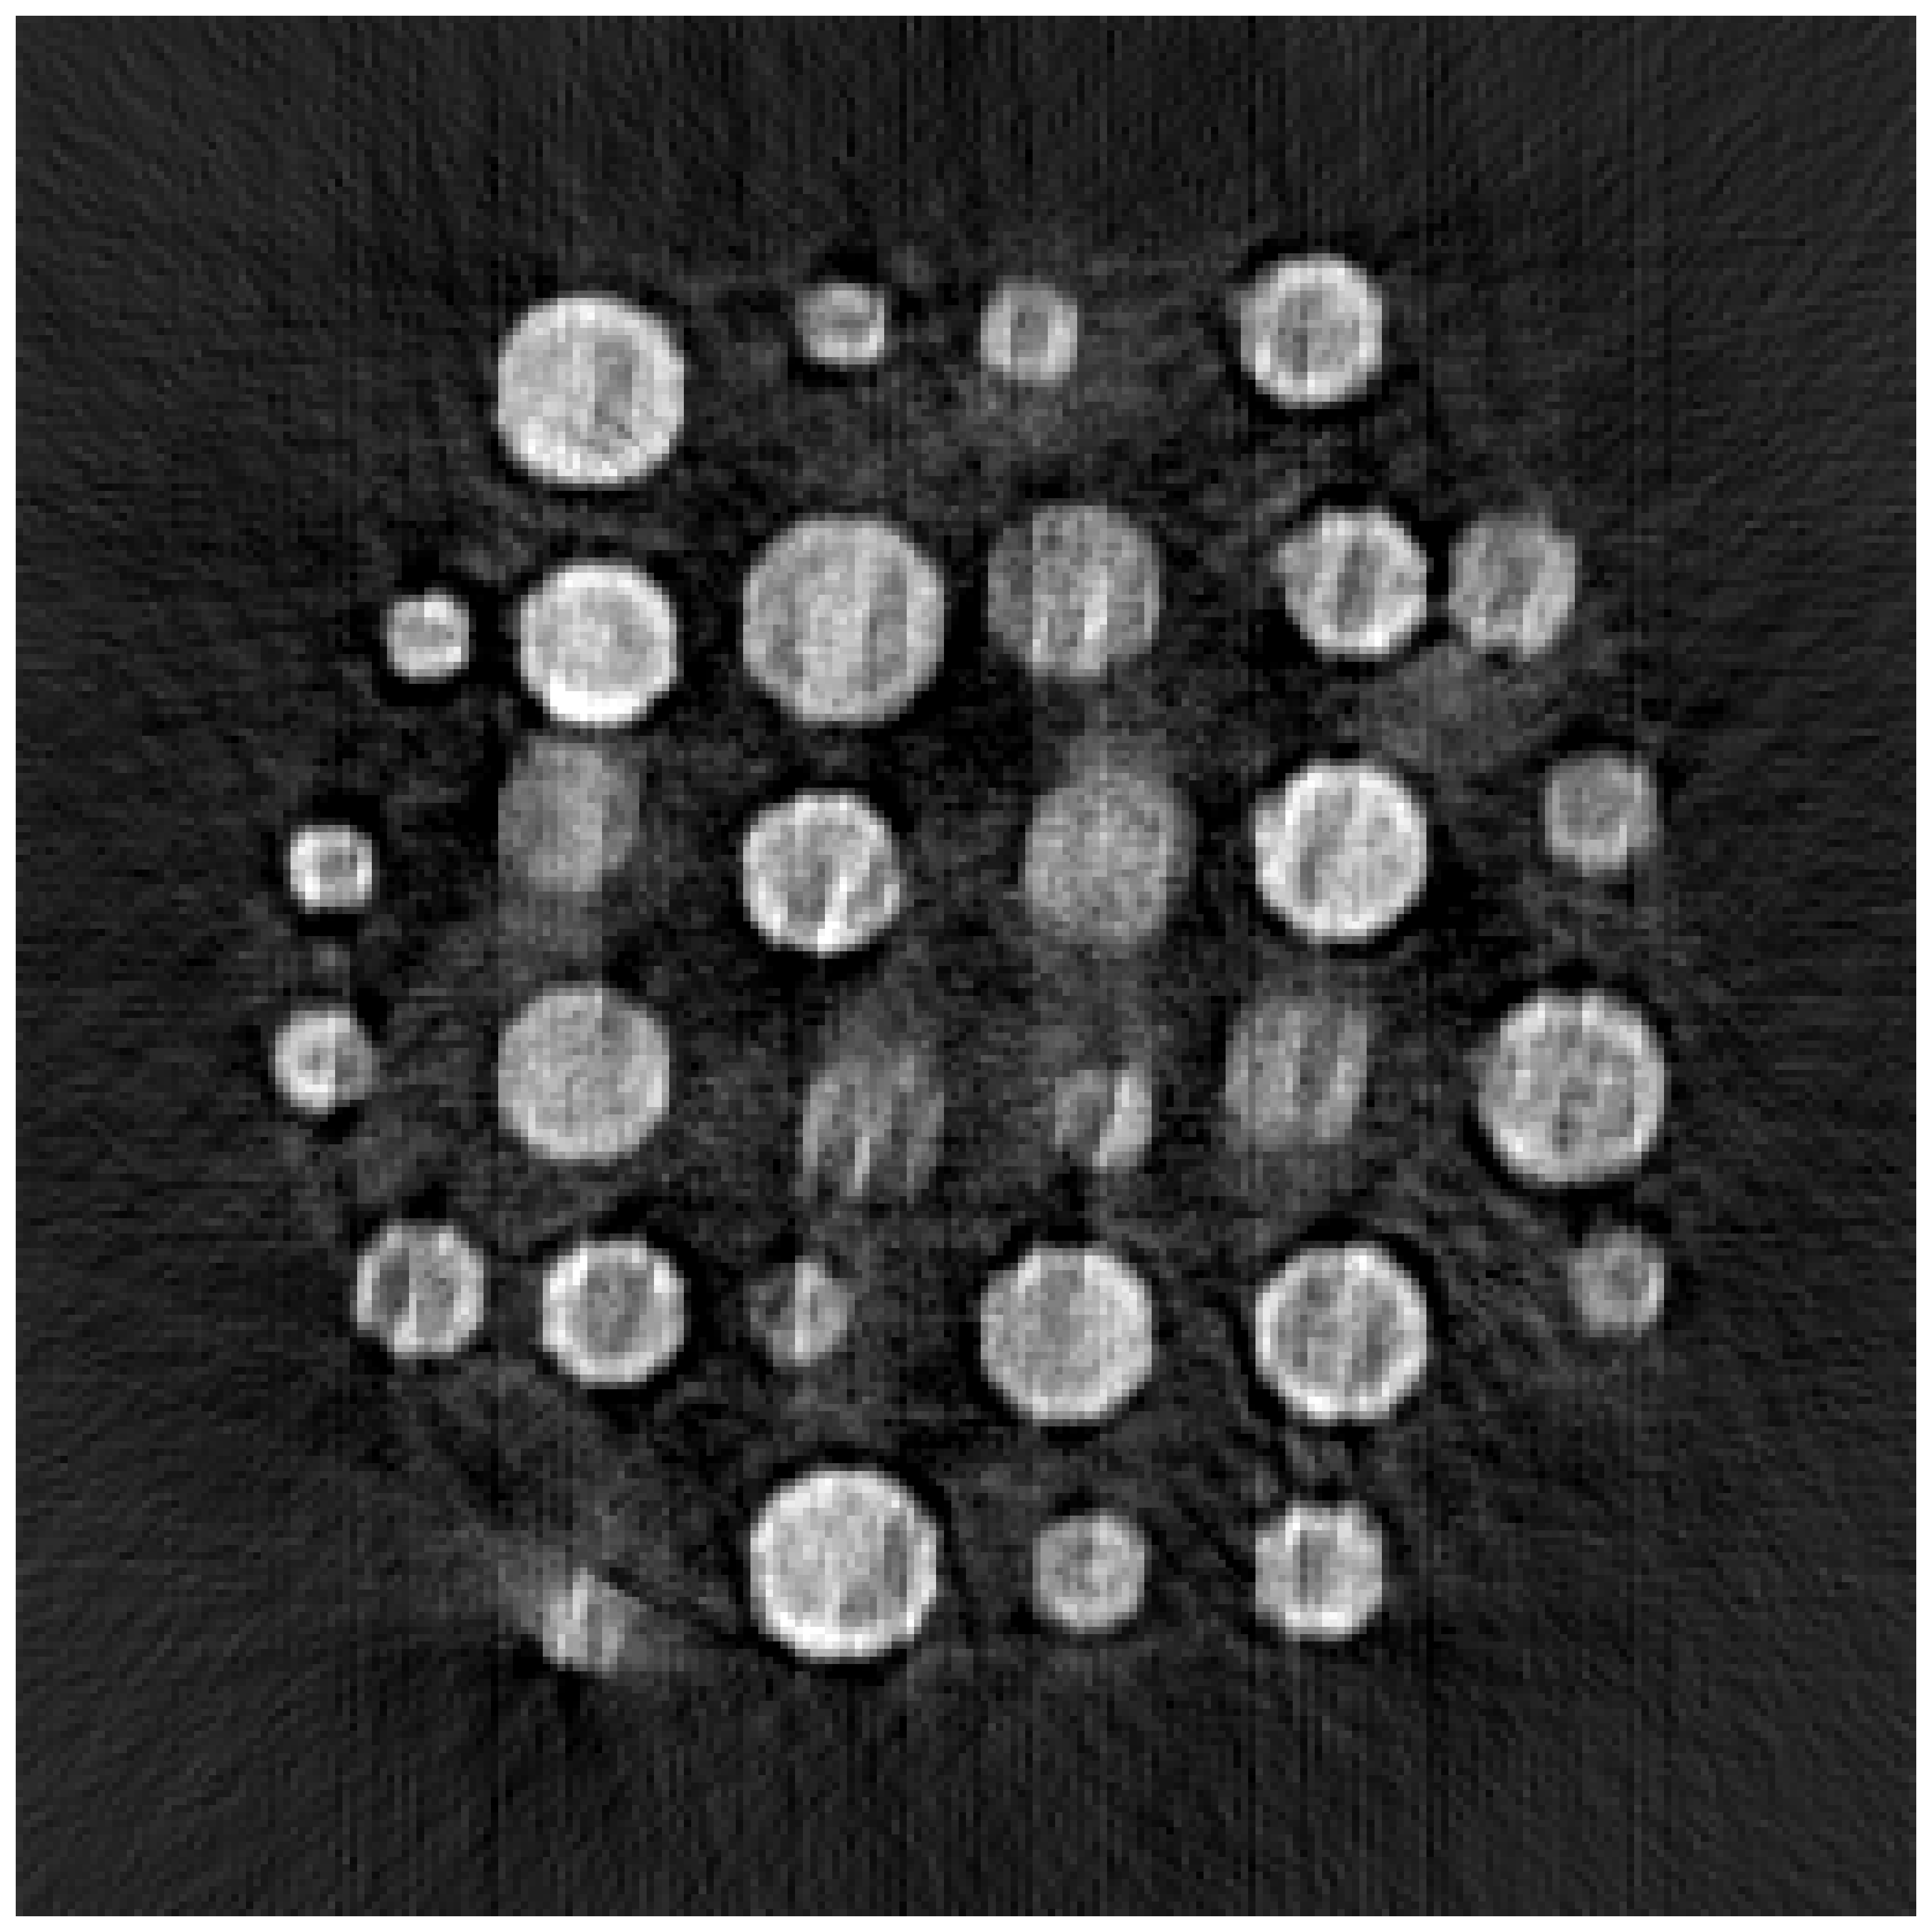
\includegraphics[width=0.15\textwidth]{ holes_gan.png}
\label{fig:holes_gan}}
\hfill
\subfloat[Difference between the image reconstructed with our method and the target reconstruction.]{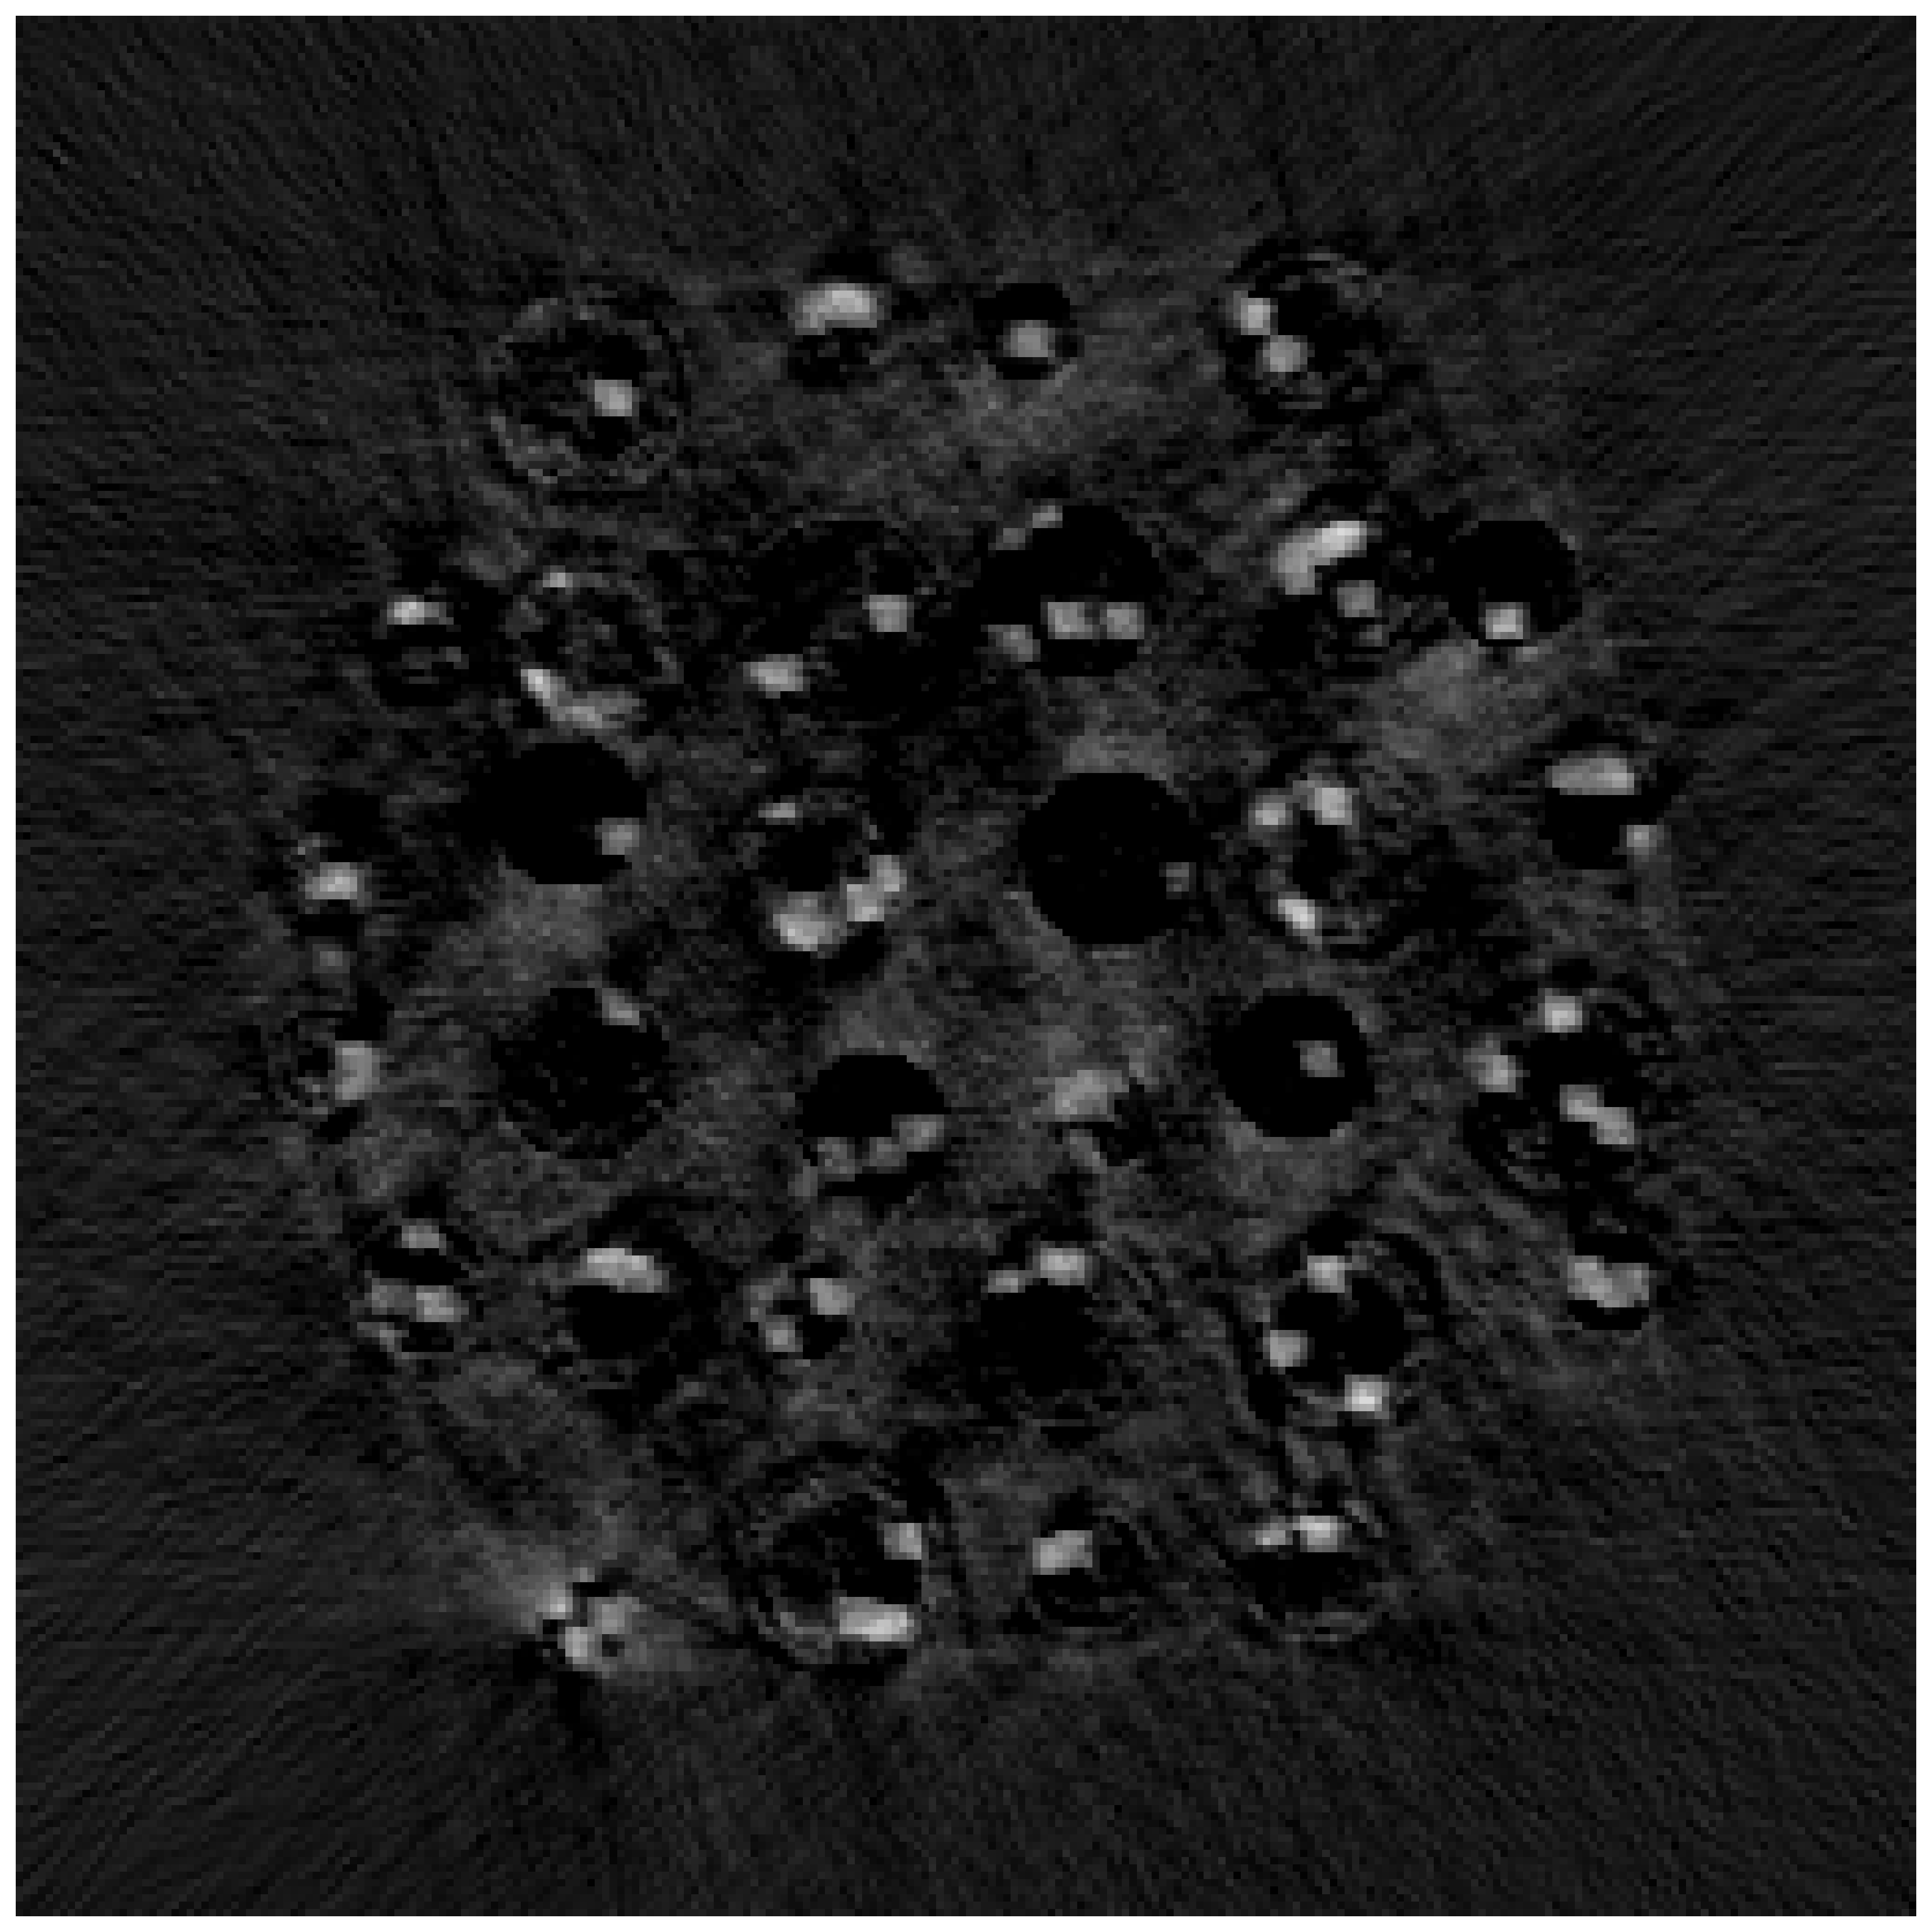
\includegraphics[width=0.15\textwidth]{ holes_gan_tar.png}
\label{fig:holes_gan_tar}}
\hfill
\subfloat[Reconstruction using the shape prior.]{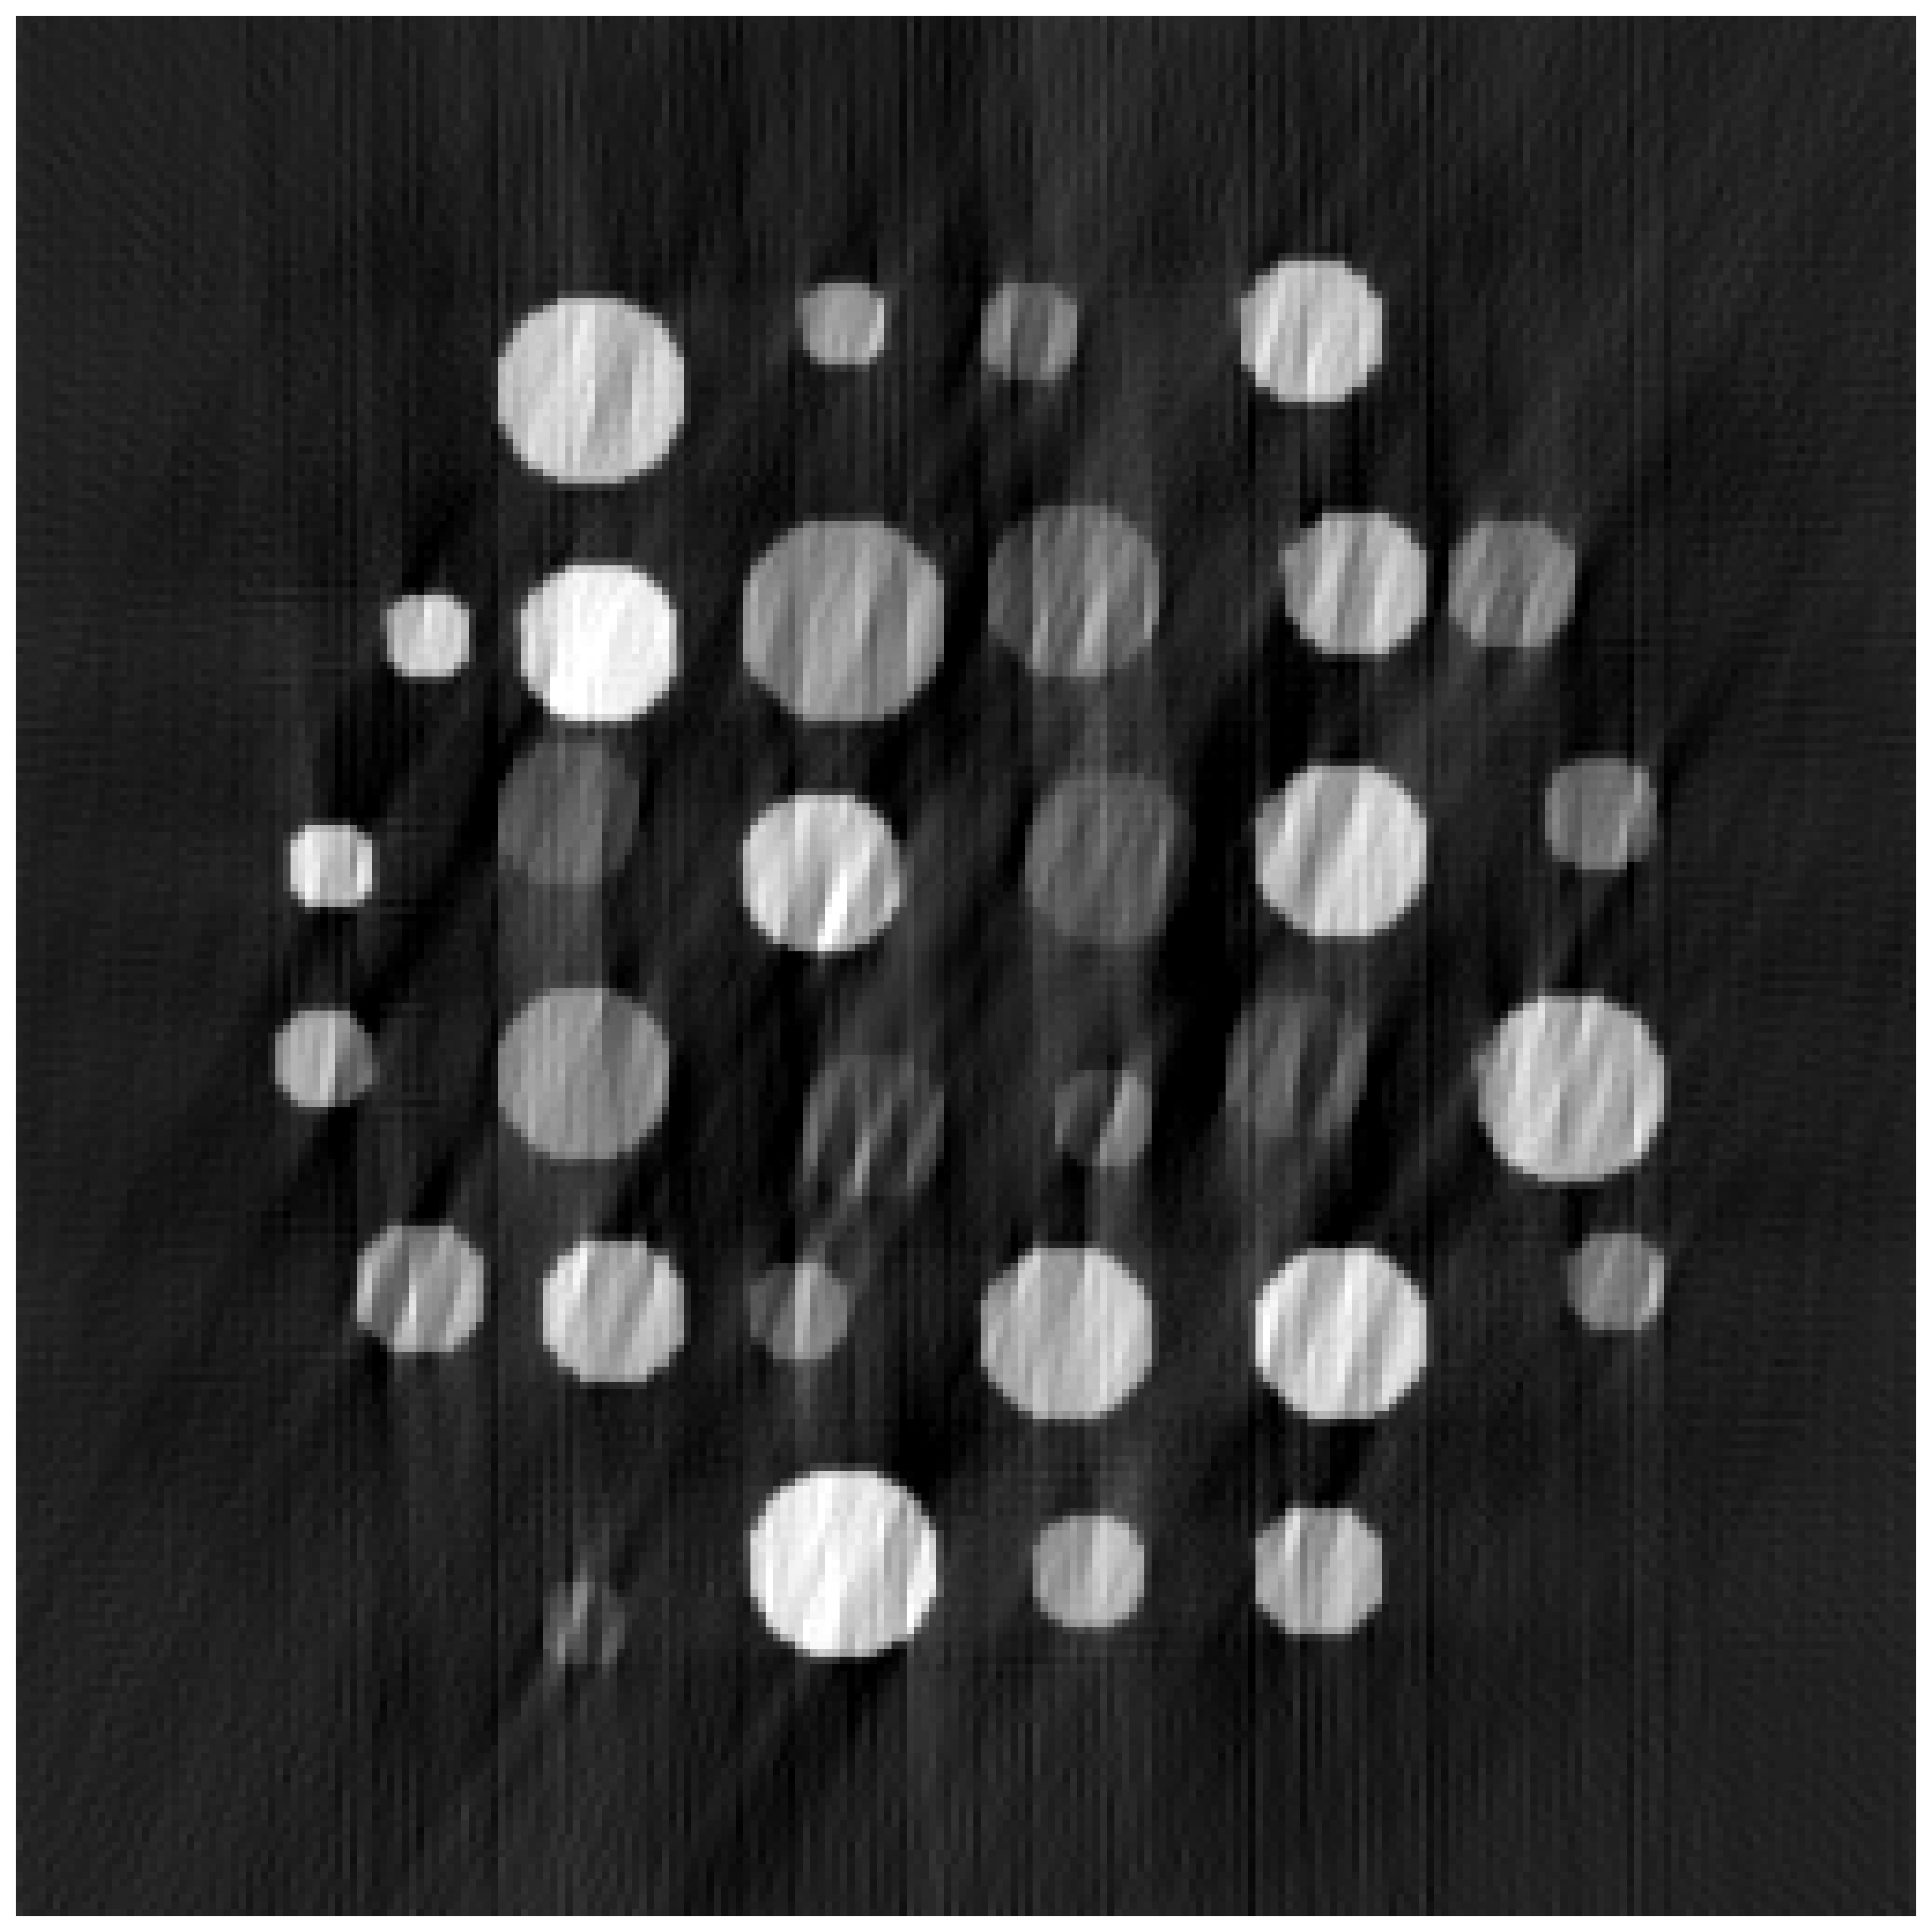
\includegraphics[width=0.15\textwidth]{ holes_cad.png}
\label{fig:holes_cad}}
\hfill
\subfloat[Difference between the image reconstructed with the shape prior and the target reconstruction.]{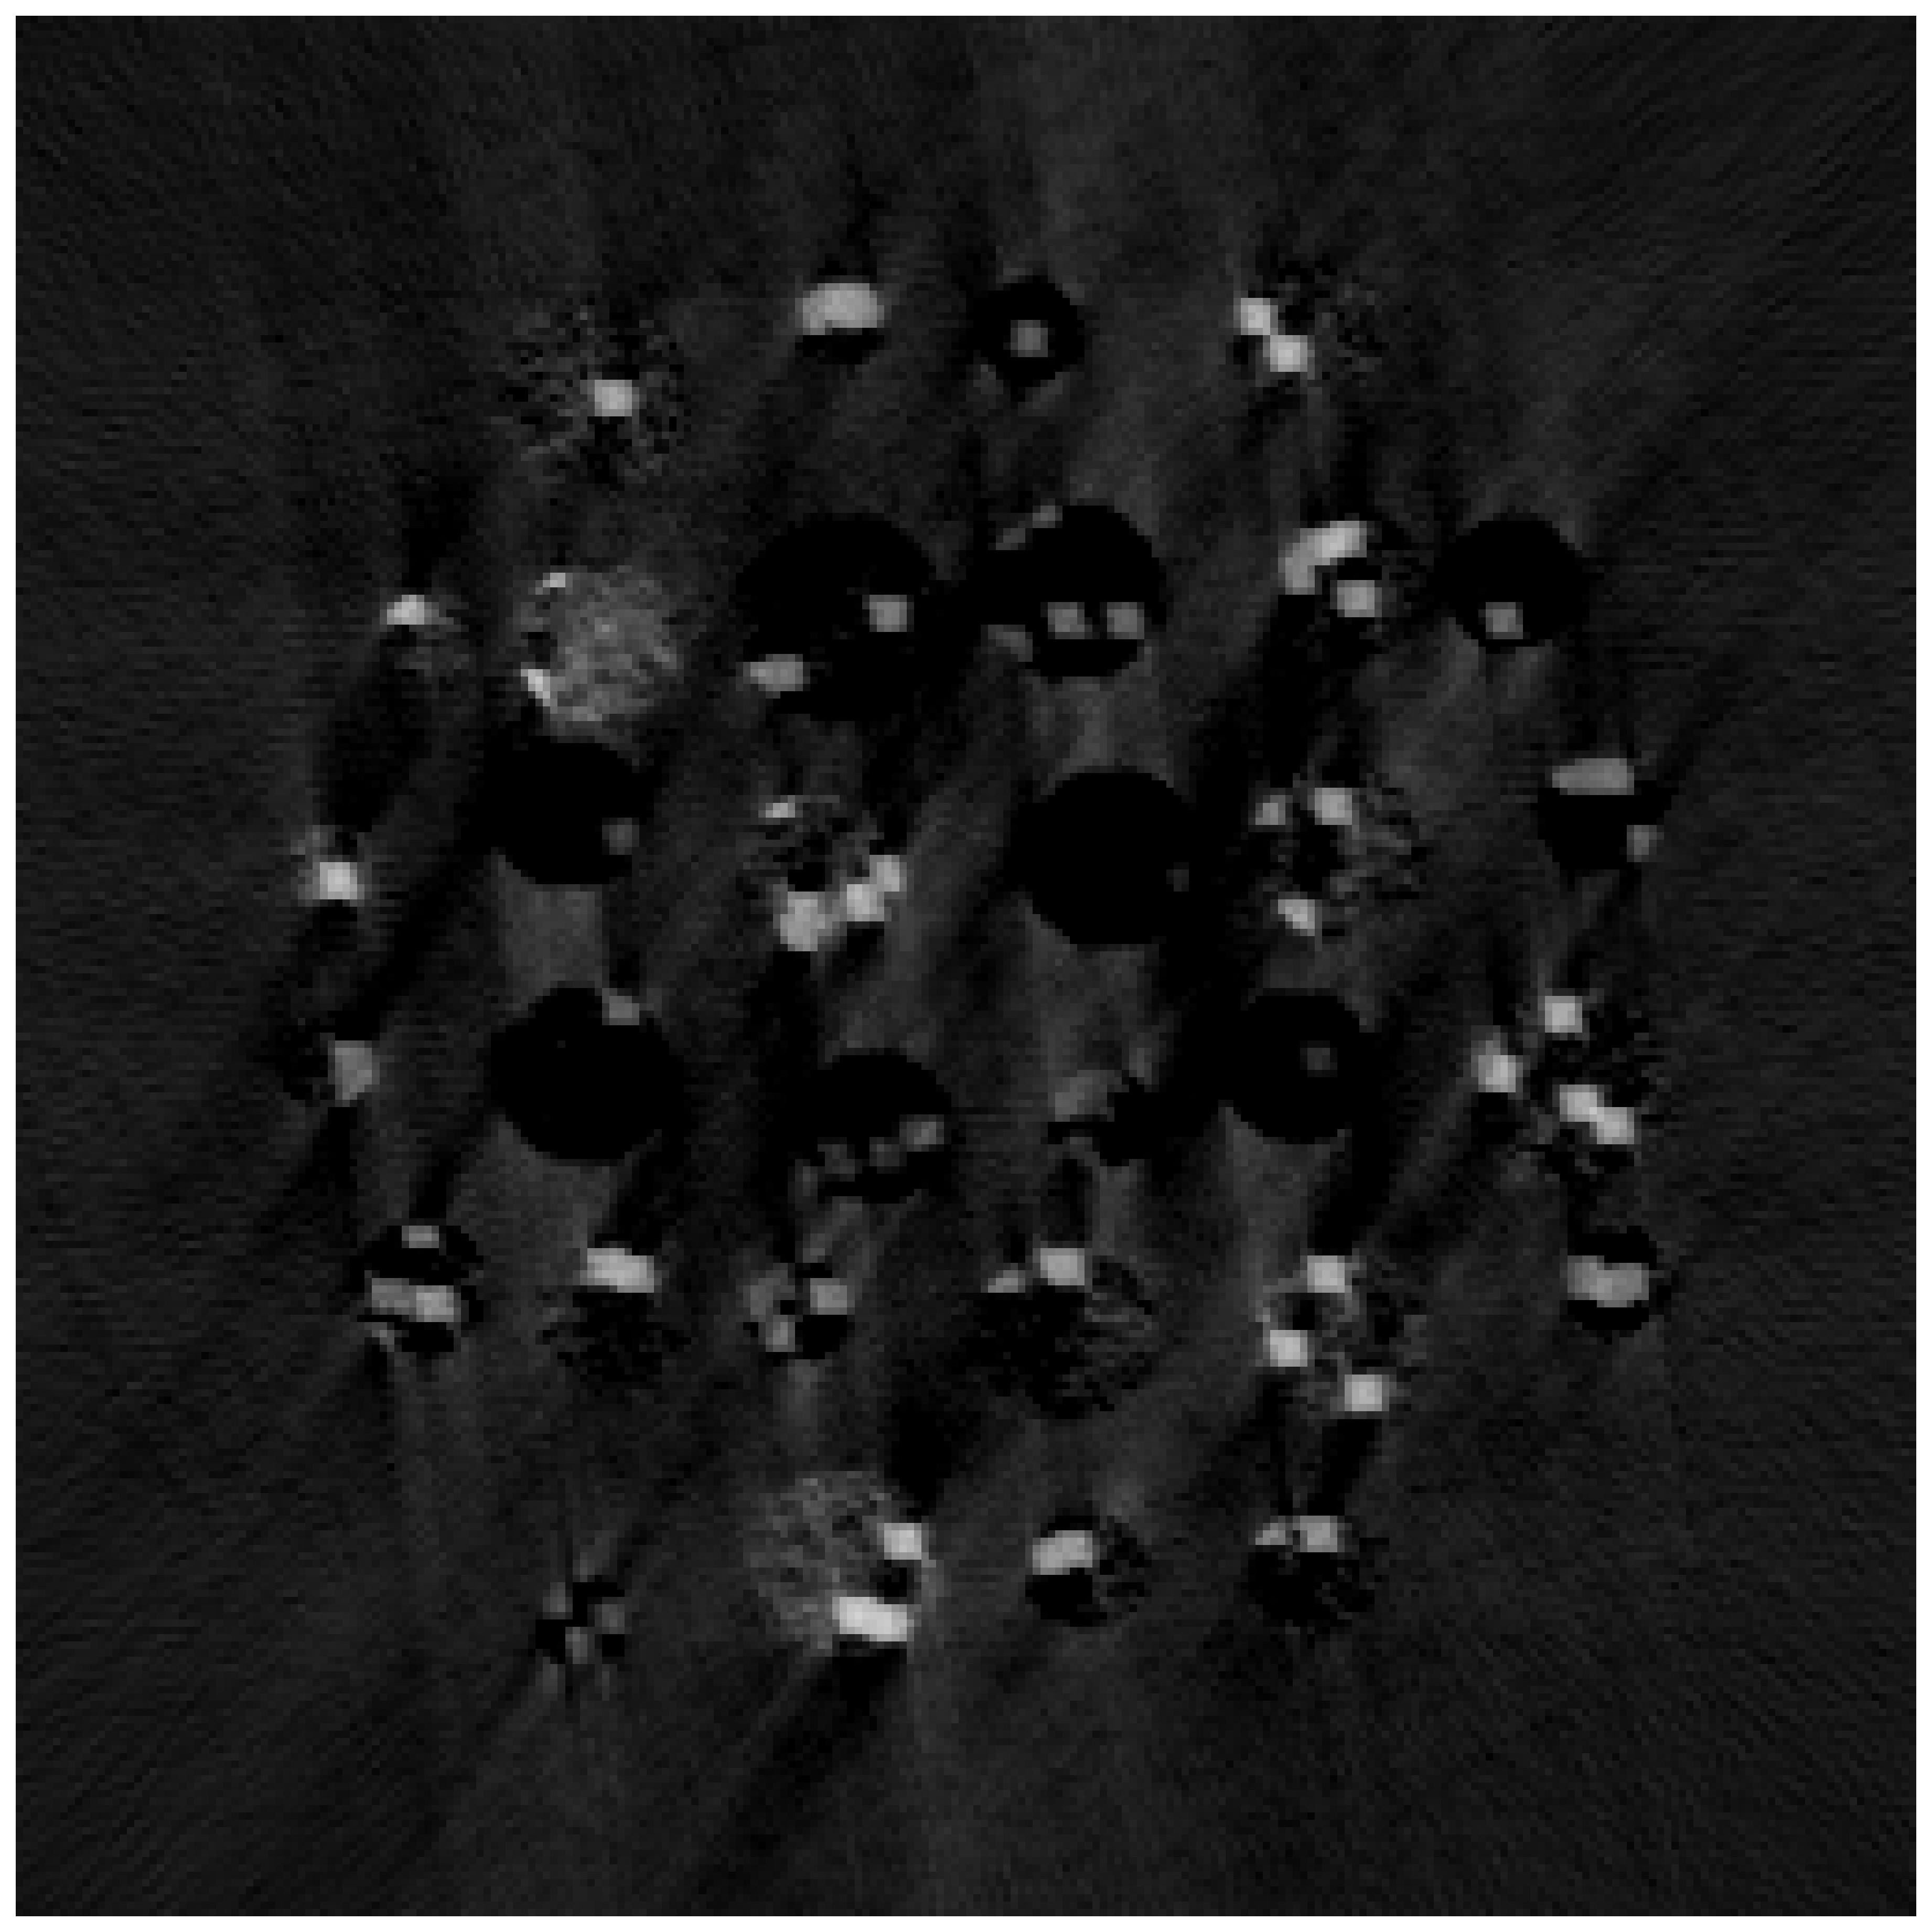
\includegraphics[width=0.15\textwidth]{ holes_cad_tar.png}
\label{fig:holes_cad_tar}}
\caption{Understanding the action of the GAN on objects with internal defects not expected by the shape prior. (\ref{fig:holes_tar}) shows the target reconstruction, (\ref{fig:holes_gan}) shows the reconstruction with our method and (\ref{fig:holes_gan_tar}) shows the difference between (\ref{fig:holes_gan}) and (\ref{fig:holes_tar}). (\ref{fig:holes_cad}) shows the reconstruction with the shape prior and (\ref{fig:holes_cad_tar}) shows the difference between (\ref{fig:holes_cad}) and (\ref{fig:holes_tar}).}
\label{fig:images_with_holes}
        
\end{figure*}  

\end{document}

